\documentclass[12pt,t]{beamer}

\usepackage{cmap}%
\usepackage[LGR,T1]{fontenc}%
\usepackage[utf8]{inputenc}%
\usepackage{alphabeta}%
\usepackage[greek,english]{babel}%
\languageattribute{greek}{polutoniko}%
\usepackage{hyperref}%
\addto\extrasenglish{\def\figureautorefname{figure}}%
\usepackage{lmodern}%

\usepackage{xcolor}
\usepackage{mathtools}
\usepackage{mdframed}
\usepackage[inline]{enumitem}
\usepackage{natbib}
\usepackage{pdflscape}
\usepackage{stmaryrd}
\usepackage{comment}
\usepackage{ifthen}
\usepackage{tikz}
\usepackage{tikz-qtree}
\usepackage{textcomp}

\usepackage{amsmath, amscd, amsthm, amssymb, mathrsfs, amsfonts, wasysym}%
\let\oldemptyset\emptyset%
\let\emptyset\varnothing%
\usepackage{cancel}%

\usepackage{tabularx}%
\usepackage{multirow}%
\renewcommand{\arraystretch}{3}%

\usepackage{pict2e}
\usepackage{picture}

\newcommand{\varslash}{%
  \mathbin{\mathpalette\pictslash{{0}{1}}}%
}
\newcommand{\varbslash}{%
  \mathbin{\mathpalette\pictslash{{1}{-1}}}%
}

\makeatletter
\newcommand{\pictslash}[2]{%
  \vcenter{%
    \sbox0{$\m@th#1\varobslash$}\dimen0=.55\wd0
    \hbox to\wd 0{%
      \hfil\pictslash@aux#2\hfil
    }%
  }%
}
\newcommand{\pictslash@aux}[2]{%
    \begin{picture}(\dimen0,\dimen0)
    \roundcap
    \linethickness{.15ex}
    \put(0,#1\dimen0){\line(1,#2){\dimen0}}
    \end{picture}%
}
\makeatother

\def\downmapsto{\rotatebox[origin=c]{270}{\ensuremath{\mapsto}}}%

\usepackage{bussproofs}%
\EnableBpAbbreviations%
\def\fCenter  {\mathbin{\vdash}}%
\def\la       {\leftarrow}%
\def\ra       {\rightarrow}%
\def\impl     {\mathbin{\slash}}%
\def\impr     {\mathbin{\backslash}}%
\def\prod     {\bullet}%
\def\prodl    {\bullet}%
\def\prodr    {\bullet}%
\def\himpl    {\!\!\fatslash\:}%
\def\himpr    {\fatbslash}%
\def\hprod    {\mathbin{\circ}}%
\def\hprodl   {\mathbin{\circ}}%
\def\hprodr   {\mathbin{\circ}}%
\def\trace    {\ensuremath{\text{trace}}}%
\def\unit     {\ensuremath{\mathbf{I}}}%
\def\sq       {\ensuremath{\Box}}%
\def\di       {\ensuremath{\Diamond}}%
\def\diIfx    {\ensuremath{\hat{\di}}}%
\def\sqIfx    {\ensuremath{\hat{\sq}}}%
\def\diExt    {\rotatebox[origin=c]{180}{\diIfx}}%
\def\sqExt    {\rotatebox[origin=c]{180}{\sqIfx}}%
\def\vsep     {\ \vert\ }%
\def\e        {\ensuremath{\mathbf{e}}}%
\def\t        {\ensuremath{\mathbf{t}}}%
\def\lamET    {\ensuremath{\lambda^{\ra}_{\{\e,\t\}}}}%
\def\S        {\text{S}}%
\def\N        {\text{N}}%
\def\NP       {\text{NP}}%
\def\PP       {\text{PP}}%
\def\INF      {\text{INF}}%
\def\A        {\text{A}}%
\def\IV       {\text{IV}}%
\def\TV       {\text{TV}}%
\def\I        {\ensuremath{\mathbf{I}}}%
\def\B        {\ensuremath{\mathbf{B}}}%
\def\C        {\ensuremath{\mathbf{C}}}%
\def\john     {\ensuremath{\text{john}}}%
\def\mary     {\ensuremath{\text{mary}}}%
\def\bill     {\ensuremath{\text{bill}}}%
\def\walks    {\ensuremath{\text{walks}}}%
\def\damned   {\ensuremath{\text{damned}}}%
\def\dog      {\ensuremath{\text{dog}}}%
\def\likes    {\ensuremath{\text{likes}}}%
\def\sees     {\ensuremath{\text{sees}}}%
\def\leave    {\ensuremath{\text{leave}}}%
\def\wants    {\ensuremath{\text{wants}}}%
\def\everyone {\ensuremath{\text{everyone}}}%
\def\different{\ensuremath{\text{different}}}%
\def\someone  {\ensuremath{\text{someone}}}%
\def\served   {\ensuremath{\text{served}}}%
\def\a        {\ensuremath{\text{a}}}%
\def\waiter   {\ensuremath{\text{waiter}}}%
\def\JOHN     {\ensuremath{\mathbf{john}}}%
\def\PERSON   {\ensuremath{\mathbf{person}}}%
\def\WAITER   {\ensuremath{\mathbf{waiter}}}%
\def\WALK     {\ensuremath{\mathbf{walk}}}%
\def\LIKE     {\ensuremath{\mathbf{like}}}%
\def\SERVE    {\ensuremath{\mathbf{serve}}}%
\def\SEE      {\ensuremath{\mathbf{see}}}%
\def\DAMN     {\ensuremath{\mathbf{damn}}}%
\def\PAST     {\ensuremath{\mathbf{past}}}%
\def\DOG      {\ensuremath{\mathbf{dog}}}%
\def\WANT     {\ensuremath{\mathbf{want}}}%
\def\plug     {\ensuremath{\:\cdot\:[\:\cdot\:]}}%
\def\qdown    {\ensuremath{\mathbf{Q}{\downarrow}}}
\def\qup      {\ensuremath{\mathbf{Q}{\uparrow}}}

\newcommand{\q}       [1][{\cdot}]{\mathbf{Q}(#1)}%
\newcommand{\focus}   [1]{\boxed{#1}}%
\newcommand{\struct}  [1]{{\cdot}#1{\cdot}}%
\newcommand{\sub}     [3]{#1[#2/#3]}%
\newcommand{\tr}      [1][({\cdot})]{#1^*}%
\newcommand{\trd}     [1][({\cdot})]{#1^{**}}%
\newcommand{\case}    [4]{\text{case}\;#1\;\text{of}\;(#2, #3)\ra#4}%
\newcommand{\add}     [2]{#1 + #2}
\newcommand{\mathplus}[0]{+}

\renewcommand*{\&}{%
  \relax
  \ifmmode
    \mathbin{\char`\&}%
  \else
    \char`\&\relax
  \fi
}

\newenvironment{pfbox}[1][0.9]%
  {\gdef\scalefactor{#1} \leavevmode\hbox\bgroup}
  {\scalebox{\scalefactor}{\DisplayProof} \egroup}

\newenvironment{pfblock}[1][0.9]%
  {\gdef\scalefactor{#1}\begin{center}\proofSkipAmount \leavevmode}%
  {\scalebox{\scalefactor}{\DisplayProof}\proofSkipAmount \end{center} }

\newboolean{notes}%
\setboolean{notes}{true}%
\providecommand{\todo}[1]{%
  \ifthenelse%
  {\boolean{notes}}%
  {\textcolor{red}{\_}\marginpar{\color{red}#1}}%
  {}}
\providecommand{\note}[1]{%
  \ifthenelse%
  {\boolean{notes}}%
  {{\color{green}\textbf{NOTE:~}#1}}%
  {}}


% rules from the Haskell code
\newcommand{\AxR}[1]{\AXC{}\RightLabel{Ax$^L$}\UIC{$#1$}}%
\newcommand{\AxL}[1]{\AXC{}\RightLabel{Ax$^R$}\UIC{$#1$}}%
\newcommand{\UnfR}[1]{\RightLabel{Foc$^R'$}\UIC{$#1$}}%
\newcommand{\UnfL}[1]{\RightLabel{Foc$^L'$}\UIC{$#1$}}%
\newcommand{\FocR}[1]{\RightLabel{Foc$^R$}\UIC{$#1$}}%
\newcommand{\FocL}[1]{\RightLabel{Foc$^L$}\UIC{$#1$}}%
\newcommand{\WithL}[2]{\RightLabel{\&L$_{#1}$}\UIC{$#2$}}%
\newcommand{\WithR}[1]{\RightLabel{\&R}\BIC{$#1$}}%
\newcommand{\ImpRL}[1]{\RightLabel{$\impr$L}\BIC{$#1$}}%
\newcommand{\ImpRR}[1]{\RightLabel{$\impr$R}\UIC{$#1$}}%
\newcommand{\ImpLL}[1]{\RightLabel{$\impl$L}\BIC{$#1$}}%
\newcommand{\ImpLR}[1]{\RightLabel{$\impl$R}\UIC{$#1$}}%
\newcommand{\Res}[3]{%
  \RightLabel{%
    \ifstrequal{1}{#1}{%
      \ifstrequal{1}{#2}{%
        Res$\impr\prod$ % Res11
      }{%
        \ifstrequal{2}{#2}{%
          Res$\prod\impr$ % Res12
        }{%
          \ifstrequal{2}{#2}{%
            Res$\impl\prod$ % Res13
          }{%
            Res$\prod\impl$ % Res14
          }
        }
      }
    }{%
      \ifstrequal{1}{#2}{%
        Res$\sq\di$ % Res21
      }{%
        Res$\di\sq$ % Res22
      }
    }
  }
  \UIC{$#3$}
}%
\newcommand{\DiaL}[1]{\RightLabel{$\di$L}\UIC{$#1$}}%
\newcommand{\DiaR}[1]{\RightLabel{$\di$R}\UIC{$#1$}}%
\newcommand{\BoxL}[1]{\RightLabel{$\sq$L}\UIC{$#1$}}%
\newcommand{\BoxR}[1]{\RightLabel{$\sq$R}\UIC{$#1$}}%
\newcommand{\IfxRR}[1]{\RightLabel{$\Ifx$RR}\UIC{$#1$}}%
\newcommand{\IfxLR}[1]{\RightLabel{$\Ifx$LR}\UIC{$#1$}}%
\newcommand{\IfxLL}[1]{\RightLabel{$\Ifx$LL}\UIC{$#1$}}%
\newcommand{\IfxRL}[1]{\RightLabel{$\Ifx$RL}\UIC{$#1$}}%
\newcommand{\ExtRR}[1]{\RightLabel{$\Ext$RR}\UIC{$#1$}}%
\newcommand{\ExtLR}[1]{\RightLabel{$\Ext$LR}\UIC{$#1$}}%
\newcommand{\ExtLL}[1]{\RightLabel{$\Ext$LL}\UIC{$#1$}}%
\newcommand{\ExtRL}[1]{\RightLabel{$\Ext$RL}\UIC{$#1$}}%
\newcommand{\UnitRL}[1]{\RightLabel{$\I$L}\UIC{$#1$}}%
\newcommand{\UnitRR}[1]{\RightLabel{$\I$R}\UIC{$#1$}}%
\newcommand{\UnitRI}[1]{\RightLabel{$\I^-$}\UIC{$#1$}}%
\newcommand{\DnB}[1]{\RightLabel{$\B$}\UIC{$#1$}}%
\newcommand{\UpB}[1]{\RightLabel{$\B'$}\UIC{$#1$}}%
\newcommand{\DnC}[1]{\RightLabel{$\C$}\UIC{$#1$}}%
\newcommand{\UpC}[1]{\RightLabel{$\C'$}\UIC{$#1$}}%

\ifdefined\usetheme\usetheme{Boadilla}\fi
\ifdefined\usecolortheme\usecolortheme{seagull}\fi
\ifdefined\beamertemplatenavigationsymbolsempty\beamertemplatenavigationsymbolsempty\fi

\author{Pepijn Kokke}
\title{Type Theory and NLP}

\begin{document}

\maketitle

\begin{frame}
  \frametitle{An abstract NLU-pipeline}
  \vfill
  \begin{center}
    \begin{minipage}{0.3\linewidth}%
      \centering
      \framebox{Morphological}\\
      $\downarrow$\\
      \framebox{Lexical}\\
      $\downarrow$\\
      \framebox{Syntactic}\\
      $\downarrow$\\
      \framebox{Semantic}\\
      $\downarrow$\\
      \framebox{Pragmatic}\\
    \end{minipage}%
    \begin{minipage}{0.7\linewidth}%
      \centering
      ``Mary saw foxes.''\\
      $\downarrow$\\
      Mary see.PAST fox.PL\\
      $\downarrow$\\
      Mary:NP see:TV.PAST fox:NP.PL\\
      $\downarrow$\\
      Mary:NP [see:TV.PAST fox:NP.PL]\\
      $\downarrow$\\
      $\exists p.\forall x.p(x)\supset(\mathbf{fox}(x)\land\mathbf{past}(\mathbf{see}(\text{mary},x)))$\\
      $\downarrow$\\
      \ldots\footnotemark\\
    \end{minipage}
  \end{center}
  \vfill
\end{frame}

\begin{frame}
  \frametitle{A simple semantic calculus}
  \begin{alignat*}{4}
    \text{Type}       \;&A,B&&\coloneqq \e\vsep\t\vsep A\ra B\\
    \text{Term}       \;&M,N&&\coloneqq x\vsep C\vsep\lambda x.M\vsep(M\;N)\\
    \text{Constant}   \;&C  &&\coloneqq
    {\forall}\vsep{\exists}\vsep{\neg}\vsep{\supset}\vsep{\land}\vsep{\lor}\vsep\ldots
  \end{alignat*}
  \\[\baselineskip]
  \begin{center}
    \begin{pfbox}[0.9]
      \AXC{$(x : A)\in Γ$} \RightLabel{{Ax}} \UIC{$Γ\fCenter x : A$}
    \end{pfbox}
    \\[\baselineskip]
    \begin{pfbox}[0.9]
      \AXC{$Γ,x : A\fCenter M : B$} \RightLabel{$\ra${I}}
      \UIC{$Γ\fCenter \lambda x.M : A\ra B$}
    \end{pfbox}
    \begin{pfbox}[0.9]
      \AXC{$Γ\fCenter M : A\ra B$} \AXC{$Γ\fCenter N : A$}
      \RightLabel{$\ra${E}} \BIC{$Γ\fCenter (M\;N) : B$}
    \end{pfbox}
  \end{center}
\end{frame}

\begin{frame}
  \frametitle{An example}
  \centering
  \vfill
  \begin{pfbox}[0.9]
    \AXC{saw}
    \RightLabel{Ax}
    \UIC{$\e,\e\e\t,\e\fCenter\e\e\t$}
    \AXC{%
      \only<1,4>{foxes}%
      \only<2,3>{mary}%
    }
    \RightLabel{Ax}
    \UIC{$\e,\e\e\t,\e\fCenter\e$}
    \RightLabel{$\ra$E}
    \BIC{$\e,\e\e\t,\e\fCenter\e\t$}
    \AXC{%
      \only<1,3>{mary}%
      \only<2,4>{foxes}%
    }
    \RightLabel{Ax}
    \UIC{$\e,\e\e\t,\e\fCenter\e$}
    \RightLabel{$\ra$E}
    \BIC{$\e,\e\e\t,\e\fCenter\t$}
  \end{pfbox}
  \\[1\baselineskip]
  $\Downarrow$
  \\[1\baselineskip]
  \onslide<1-4>{%
  $\text{mary}:\e,\text{saw}:\e\e\t,\text{foxes}:\e
  \fCenter((\text{saw}\;\text{foxes})\;\text{mary}):\t$
  }
  \onslide<2-4>{%
  $\text{mary}:\e,\text{saw}:\e\e\t,\text{foxes}:\e
  \fCenter((\text{saw}\;\text{mary})\;\text{foxes}):\t$
  }
  \onslide<3-4>{%
  $\text{mary}:\e,\text{saw}:\e\e\t,\text{foxes}:\e
  \fCenter((\text{saw}\;\text{mary})\;\text{mary}):\t$
  }
  \onslide<4-4>{%
  $\text{mary}:\e,\text{saw}:\e\e\t,\text{foxes}:\e
  \fCenter((\text{saw}\;\text{foxes})\;\text{foxes}):\t$
  }
  \vfill
\end{frame}

\begin{frame}
  \frametitle{No implicit set structure}
  \centering
  \onslide<1>{\mdframed}\centering
  $\text{Structure}\;Γ,Δ,Π\coloneqq\emptyset\vsep A\vsepΓ\prodΔ$
  \onslide<1>{\endmdframed}
  \onslide<2>{\mdframed}\centering
    \begin{pfbox}[0.9]
      \AXC{}\RightLabel{{Ax}}\UIC{$A\fCenter A$}
    \end{pfbox}
    \\[1\baselineskip]
    \begin{pfbox}[0.9]
      \AXC{$Γ\prod A\fCenter B$} \RightLabel{$\ra${I}}
      \UIC{$Γ\fCenter A\ra B$}
    \end{pfbox}
    \begin{pfbox}[0.9]
      \AXC{$Γ\fCenter A\ra B$} \AXC{$Δ\fCenter A$}
      \RightLabel{$\ra${E}} \BIC{$Γ\prod Δ\fCenter B$}
    \end{pfbox}
  \onslide<2>{\endmdframed}
  \onslide<3>{\mdframed}\centering
    \begin{pfbox}[0.9]
      \AXC{$Σ[Γ\prod Γ]\fCenter B$} \RightLabel{Cont.}
      \UIC{$Σ[Γ]\fCenter B$}
    \end{pfbox}
    \begin{pfbox}[0.9]
      \AXC{$Σ[Γ]\fCenter B$} \RightLabel{Weak.}
      \UIC{$Σ[Γ\prod Δ]\fCenter B$}
    \end{pfbox}
    \\[1\baselineskip]
    \begin{pfbox}[0.9]
      \AXC{$Σ[Γ\prod \emptyset]\fCenter B$}
      \RightLabel{$\emptyset${E}} \UIC{$Σ[Γ]\fCenter B$}
    \end{pfbox}
    \\[1\baselineskip]
    \begin{pfbox}[0.9]
      \AXC{$Σ[Δ\prod Γ]\fCenter B$} \RightLabel{Comm.}
      \UIC{$Σ[Γ\prod Δ]\fCenter B$}
    \end{pfbox}
    \begin{pfbox}[0.9]
      \AXC{$Σ[(Γ\prod Δ)\prod Π]\fCenter B$}
      \doubleLine\RightLabel{Ass.}
      \UIC{$Σ[Γ\prod (Δ\prod Π)]\fCenter B$}
    \end{pfbox}
  \onslide<3>{\endmdframed}
  \note{%
    The first section contains just the logical rules that we had
    before, albeit now defined with binary trees instead of sets. The
    second section contains a new set of structural rules, which
    emulate the structure of set membership. We have weakening and
    contraction, which express the ideas that if A is in X, then A is
    still in X with new formulas added, or with duplicates
    removed. Then secondly, we have $\emptyset$E, associativity and
    commutativity, which together express the idea that order is
    irrelevant.

    Now, we're not going to prove this, but I'm sure you all can see
    that these two calculi are equivalent. This means that we can
    label these inference rules with the terms of the calculus on the
    previous slide. The term labelling of the logical rules is exactly
    as before; the term labelling of the structural rules is
    uninteresting, as they do not actually change anything in the
    term. The only exception to this is contraction: the types in the
    first and the second Γ have different names (say $y_0$ to $y_i$
    and $z_0$ to $z_i$) which have to be point-wise relabelled (to say
    $x_0$ to $x_i$).
  }
\end{frame}

\begin{frame}
  \frametitle{An example}
  \centering
  \vfill
  \only<1>{%
    \begin{pfbox}[0.9]
      \AXC{saw}\RightLabel{Ax}\UIC{$\e\e\t\fCenter\e\e\t$}
      \AXC{foxes}\RightLabel{Ax}\UIC{${\color{green}\e}\fCenter\e$}
      \RightLabel{$\ra$E}
      \BIC{$\e\e\t\prod{\color{green}\e}\fCenter\e\t$}
      \AXC{mary}\RightLabel{Ax}\UIC{${\color{red}\e}\fCenter\e$}
      \RightLabel{$\ra$E}
      \BIC{$(\e\e\t\prod{\color{green}\e})\prod{\color{red}\e}\fCenter\e\t$}
      \RightLabel{Comm.}
      \UIC{${\color{red}\e}\prod(\e\e\t\prod{\color{green}\e})\fCenter\e\t$}
    \end{pfbox}
    \\[1\baselineskip]
    $\Downarrow$
    \\[1\baselineskip]
    $\text{mary}:\e,\text{saw}:\e\e\t,\text{foxes}:\e
    \fCenter((\text{saw}\;\text{foxes})\;\text{mary}):\t$
  }
  \only<2>{%
    \begin{pfbox}[0.9]
      \AXC{saw}\RightLabel{Ax}\UIC{$\e\e\t\fCenter\e\e\t$}
      \AXC{mary}\RightLabel{Ax}\UIC{${\color{red}\e}\fCenter\e$}
      \RightLabel{$\ra$E}
      \BIC{$\e\e\t\prod{\color{red}\e}\fCenter\e\t$}
      \AXC{foxes}\RightLabel{Ax}\UIC{${\color{green}\e}\fCenter\e$}
      \RightLabel{$\ra$E}
      \BIC{$(\e\e\t\prod{\color{red}\e})\prod{\color{green}\e}\fCenter\e\t$}
      \RightLabel{Comm.}
      \UIC{$({\color{red}\e}\prod\e\e\t)\prod{\color{green}\e}\fCenter\e\t$}
      \RightLabel{Ass.}
      \UIC{${\color{red}\e}\prod(\e\e\t\prod{\color{green}\e})\fCenter\e\t$}
    \end{pfbox}
    \\[1\baselineskip]
    $\Downarrow$
    \\[1\baselineskip]
    $\text{mary}:\e,\text{saw}:\e\e\t,\text{foxes}:\e
    \fCenter((\text{saw}\;\text{mary})\;\text{foxes}):\t$
  }
  \only<3>{%
    \begin{pfbox}[0.9]
      \AXC{saw}\RightLabel{Ax}\UIC{$\e\e\t\fCenter\e\e\t$}
      \AXC{mary}\RightLabel{Ax}\UIC{${\color{red}\e}\fCenter\e$}
      \RightLabel{$\ra$E}
      \BIC{$\e\e\t\prod{\color{red}\e}\fCenter\e\t$}
      \AXC{mary}\RightLabel{Ax}\UIC{${\color{red}\e}\fCenter\e$}
      \RightLabel{$\ra$E}
      \BIC{$(\e\e\t\prod{\color{red}\e})\prod{\color{red}\e}\fCenter\e\t$}
      \RightLabel{Ass.}
      \UIC{$\e\e\t\prod({\color{red}\e}\prod{\color{red}\e})\fCenter\e\t$}
      \RightLabel{Comm.}
      \UIC{$({\color{red}\e}\prod{\color{red}\e})\prod\e\e\t\fCenter\e\t$}
      \RightLabel{Cont.}
      \UIC{${\color{red}\e}\prod\e\e\t\prod\fCenter\e\t$}
      \RightLabel{Weak.}
      \UIC{${\color{red}\e}\prod(\e\e\t\prod{\color{green}\e})\fCenter\e\t$}
    \end{pfbox}
    \\[1\baselineskip]
    $\Downarrow$
    \\[1\baselineskip]
    $\text{mary}:\e,\text{saw}:\e\e\t,\text{foxes}:\e
    \fCenter((\text{saw}\;\text{mary})\;\text{mary}):\t$
  }
  \only<4>{%
    \begin{pfbox}[0.9]
      \AXC{saw}\RightLabel{Ax}\UIC{$\e\e\t\fCenter\e\e\t$}
      \AXC{foxes}\RightLabel{Ax}\UIC{${\color{green}\e}\fCenter\e$}
      \RightLabel{$\ra$E}
      \BIC{$\e\e\t\prod{\color{green}\e}\fCenter\e\t$}
      \AXC{foxes}\RightLabel{Ax}\UIC{${\color{green}\e}\fCenter\e$}
      \RightLabel{$\ra$E}
      \BIC{$(\e\e\t\prod{\color{green}\e})\prod{\color{green}\e}\fCenter\e\t$}
      \RightLabel{Ass.}
      \UIC{$\e\e\t\prod({\color{green}\e}\prod{\color{green}\e})\fCenter\e\t$}
      \RightLabel{Cont.}
      \UIC{$\e\e\t\prod{\color{green}\e}\fCenter\e\t$}
      \RightLabel{Weak.}
      \UIC{$(\e\e\t\prod{\color{green}\e})\prod{\color{red}\e}\fCenter\e\t$}
      \RightLabel{Comm.}
      \UIC{${\color{red}\e}\prod(\e\e\t\prod{\color{green}\e})\fCenter\e\t$}
    \end{pfbox}
    \\[1\baselineskip]
    $\Downarrow$
    \\[1\baselineskip]
    $\text{mary}:\e,\text{saw}:\e\e\t,\text{foxes}:\e
    \fCenter((\text{saw}\;\text{foxes})\;\text{foxes}):\t$
  }
  \vfill
\end{frame}

\begin{frame}
  \frametitle{A simple syntactic calculus}
    \centering
    \begin{alignat*}{4}
      \text{Type}\;&A,B&&\coloneqq\S\vsep\N\vsep\NP\vsep A\impr B\vsep B\impl A\\
      \text{Structure}\;&Γ,Δ&&\coloneqq A\vsep Γ\prodΔ
    \end{alignat*}%
    \\[1\baselineskip]
    \begin{pfbox}[0.9]
      \AXC{} \RightLabel{{Ax}} \UIC{$A\fCenter A$}
    \end{pfbox}
    \\[1\baselineskip]
    \begin{pfbox}[0.9]
      \AXC{$A\prodΓ\fCenter B$} \RightLabel{$\impr${I}}
      \UIC{$Γ\fCenter A\impr B$}
    \end{pfbox}
    \begin{pfbox}[0.9]
      \AXC{$Γ\fCenter A$} \AXC{$Δ\fCenter A\impr B$} \RightLabel{$\impr${E}}
      \BIC{$Γ\prodΔ\fCenter B$}
    \end{pfbox}
    \\[1\baselineskip]
    \begin{pfbox}[0.9]
      \AXC{$Γ\prod A\fCenter B$} \RightLabel{$\impl${I}}
      \UIC{$Γ\fCenter B\impl A$}
    \end{pfbox}
    \begin{pfbox}[0.9]
      \AXC{$Γ\fCenter B\impl A$} \AXC{$Δ\fCenter A$} \RightLabel{$\impl${E}}
      \BIC{$Γ\prod Δ\fCenter B$}
    \end{pfbox}
\end{frame}

\begin{frame}
  \frametitle{An example}
  \centering
  \vfill
  \begin{pfbox}[0.9]
    \AXC{mary}
    \RightLabel{Ax}
    \UIC{$\NP\fCenter\NP$}
    \AXC{saw}
    \RightLabel{Ax}
    \UIC{$(\NP\impr\S)\impl\NP\fCenter(\NP\impr\S)\impl\NP$}
    \AXC{foxes}
    \RightLabel{Ax}
    \UIC{$\NP\fCenter\NP$}
    \RightLabel{$\impl$E}
    \BIC{$(\NP\impr\S)\impl\NP\prod\NP\fCenter\NP\impr\S$}
    \RightLabel{$\impr$E}
    \BIC{$\NP\prod((\NP\impr\S)\impl\NP\prod\NP)\fCenter\S$}
  \end{pfbox}
  \\[\baselineskip]
  $\Downarrow$
  \\[\baselineskip]
  ?
  \vfill
\end{frame}

\begin{frame}
  \frametitle{From syntactic to semantic calculus}
  \centering
  \[\!
    \fbox{\(
      \begin{aligned}
        &\tr[\S]         &&\mapsto\t      \\
        &\tr[\N]         &&\mapsto\e\ra\t \\
        &\tr[(A\impr B)] &&\mapsto\tr[A]\ra\tr[B]
      \end{aligned}
      \qquad
      \begin{aligned}
        \\
        &\tr[\NP]        &&\mapsto\e      \\
        &\tr[(B\impl A)] &&\mapsto\tr[A]\ra\tr[B]
      \end{aligned}
      \)}
  \]
  \vfill
  \only<1>{%
    \begin{pfbox}[0.9]
      \AXC{}\RightLabel{Ax}\UIC{$A\fCenter A$}
    \end{pfbox}
    $\Longrightarrow$
    \begin{pfbox}[0.9]
      \AXC{}\RightLabel{Ax}\UIC{$\tr[A]\fCenter\tr[A]$}
    \end{pfbox}
  }
  \only<2>{%
    \begin{pfbox}[0.9]
      \AXC{$A\prod Γ\fCenter B$} \RightLabel{$\impr${I}}
      \UIC{$Γ\fCenter A\impr B$}
    \end{pfbox}
    $\Longrightarrow$
    \begin{pfbox}[0.9]
      \AXC{$\tr[A]\prod\tr[Γ]\fCenter\tr[B]$} \RightLabel{Comm.}
      \UIC{$\tr[Γ]\prod\tr[A]\fCenter\tr[B]$} \RightLabel{$\ra$I}
      \UIC{$\tr[Γ]\fCenter\tr[A]\ra\tr[B]$}
    \end{pfbox}
    \\[1\baselineskip]
    \begin{pfbox}[0.9]
      \AXC{$Γ\prod A\fCenter B$} \RightLabel{$\impl${I}}
      \UIC{$Γ\fCenter B\impl A$}
    \end{pfbox}
    $\Longrightarrow$
    \begin{pfbox}[0.9]
      \AXC{$\tr[Γ]\prod\tr[A]\fCenter\tr[B]$} \RightLabel{$\ra$I}
      \UIC{$\tr[Γ]\fCenter\tr[A]\ra\tr[B]$}
    \end{pfbox}
  }
  \only<3>{%
    \begin{pfbox}[0.9]
      \AXC{$Γ\fCenter A$} \AXC{$Δ\fCenter A\impr B$}
      \RightLabel{$\impr${E}} \BIC{$Γ\prod Δ\fCenter B$}
    \end{pfbox}
    $\Longrightarrow$
    \begin{pfbox}[0.9]
      \AXC{$\tr[Δ]\fCenter\tr[A]\ra\tr[B]$}
      \AXC{$\tr[Γ]\fCenter\tr[A]$} \RightLabel{$\ra${E}}
      \BIC{$\tr[Δ]\prod\tr[Γ]\fCenter\tr[B]$} \RightLabel{Comm.}
      \UIC{$\tr[Γ]\prod\tr[Δ]\fCenter\tr[B]$}
    \end{pfbox}
    \\[1\baselineskip]
    \begin{pfbox}[0.9]
      \AXC{$Γ\fCenter B\impl A$}
      \AXC{$Δ\fCenter A$} \RightLabel{$\impl${E}}
      \BIC{$Γ\prod Δ\fCenter B$}
    \end{pfbox}
    $\Longrightarrow$
    \begin{pfbox}[0.9]
      \AXC{$\tr[Γ]\fCenter\tr[A]\ra\tr[B]$}
      \AXC{$\tr[Δ]\fCenter\tr[A]$} \RightLabel{$\ra${E}}
      \BIC{$\tr[Γ]\prod\tr[Δ]\fCenter\tr[B]$}
    \end{pfbox}
  }
  \vfill
\end{frame}

\begin{frame}
  \frametitle{An example}
  \centering
  \vfill
  \begin{pfbox}[0.9]
    \AXC{mary}
    \RightLabel{Ax}
    \UIC{$\NP\fCenter\NP$}
    \AXC{saw}
    \RightLabel{Ax}
    \UIC{$(\NP\impr\S)\impl\NP\fCenter(\NP\impr\S)\impl\NP$}
    \AXC{foxes}
    \RightLabel{Ax}
    \UIC{$\NP\fCenter\NP$}
    \RightLabel{$\impl$E}
    \BIC{$(\NP\impr\S)\impl\NP\prod\NP\fCenter\NP\impr\S$}
    \RightLabel{$\impr$E}
    \BIC{$\NP\prod((\NP\impr\S)\impl\NP\prod\NP)\fCenter\S$}
  \end{pfbox}
  \\[1\baselineskip]
  $\Downarrow$
  \\[1\baselineskip]
  $\text{mary}:\e,\text{saw}:\e\e\t,\text{foxes}:\e
  \fCenter((\text{saw}\;\text{foxes})\;\text{mary}):\t$
  \vfill
\end{frame}

\begin{frame}
  \frametitle{Joachim Lambek (1922--2014)}
  \centering
  \vspace*{-5ex}
  \includegraphics[height=\paperheight]{lambek.pdf}
  \note{%
    Now, most of the work above is due to Lambek, outlined in two
    papers published in '58 and '61. There was one distinction,
    though. Lambek used a sequent calculus, instead of a natural
    deduction system, because this will give us an easy proof search
    procedure. We want that too. But we won't settle for just
    using a sequent calculus system. We want to use a modern
    approach.
  }
\end{frame}

\begin{frame}
  \frametitle{Display calculus}
  \vfill
  \only<1>{%
    \begin{itemize}
    \item Generalises the sequent calculus;
    \item Generic proof of cut-elimination;
      \vspace*{1\baselineskip}
      \begin{center}
        \begin{pfbox}[0.9]
          \AXC{$Γ\fCenter A$} \AXC{$A\fCenter Δ$} \RightLabel{Cut}
          \BIC{$Γ\fCenter Δ$}
        \end{pfbox}
      \end{center}
      \vspace*{1\baselineskip}
      \note{%
        This is a big deal. Because cut is a big with. If cut is added
        as a rule, then we lose the sub-formula property, which means,
        amongst others, that we lose decidable proof search. But if we
        get rid of the cut rule, then we no longer have a logic, as
        logics are reflexive, transitive relations. In addition, there
        is a belief that `cut' represents an important property of
        language -- namely the ability to substitute things of the
        same type, i.e. if something is a noun phrase, we can use it
        anywhere that we can use a noun phrase. What this theorem
        gives us is the certainty that, whatever we connectives or
        rules we add to our system, as long as they obey the rules of
        display calculus, we will keep cut elimination. And we're
        going to be adding a lot of things.
      }
    \item Decidable, easy-to-implement proof search;
      \note{%
        Display calculus has a very simple proof search procedure:
        naive backward-chaining search. Start out with your goal
        sequent, check which rules you can apply, apply them and
        repeat. Because logical rule is guaranteed to remove a
        connective, this is decidable and complete. All we need to
        add, is a check to see if we've made a loop, and if so, also
        terminate.
      }
    \item Focusing can be used to restrict spurious ambiguity.
      \note{%
        Lastly, it is a well known fact that sequent calculus proofs
        and natural deduction proofs don't neatly map one-to-one. In
        fact, there is a many-to-one relationship, with many sequent
        calculus proofs mapping to a single natural deduction
        proof. Display calculus has this property as well. However, we
        can cull the proof space to remove most spurious ambiguity
        using a technique called focusing. We won't go into this for
        this presentation, though.
      }
    \end{itemize}
  }
  \only<2-4>{%
    \onslide<2>{\mdframed}\centering
    \(\!
    \begin{aligned}
      \text{Structure}&^+\;Γ&&\coloneqq\struct{A}\vsepΓ_1\prod Γ_2\\
      \text{Structure}&^-\;Δ&&\coloneqq\struct{A}\vsepΓ\imprΔ\vsepΔ\implΓ
    \end{aligned}\)
    \onslide<2>{\endmdframed}
    \onslide<3>{\mdframed}\centering
    \begin{pfbox}[0.9]
      \AXC{}
      \RightLabel{Ax}
      \UIC{$\struct{A}\fCenter\struct{A}$}
    \end{pfbox}
    \\[1\baselineskip]
    \begin{pfbox}[0.9]
      \AXC{$Γ\fCenter\struct{A}$}
      \AXC{$\struct{B}\fCenter Δ$}
      \RightLabel{L$\impr$}
      \BIC{$\struct{A\impr B}\fCenter Γ\impr Δ$}
    \end{pfbox}
    \begin{pfbox}[0.9]
      \AXC{$Γ\fCenter\struct{A}\impr\struct{B}$}
      \RightLabel{R$\impr$}
      \UIC{$Γ\fCenter\struct{A\impr B}$}
    \end{pfbox}
    \\[1\baselineskip]
    \begin{pfbox}[0.9]
      \AXC{$Γ\fCenter\struct{A}$}
      \AXC{$\struct{B}\fCenter Δ$}
      \RightLabel{L$\impl$}
      \BIC{$\struct{B\impl A}\fCenter Δ\impl Γ$}
    \end{pfbox}
    \begin{pfbox}[0.9]
      \AXC{$Γ\fCenter\struct{B}\impl\struct{A}$}
      \RightLabel{R$\impl$}
      \UIC{$Γ\fCenter\struct{B\impl A}$}
    \end{pfbox}
    \onslide<3>{\endmdframed}
    \onslide<4>{\mdframed}\centering
    \begin{pfbox}[0.9]
      \AXC{$Γ_2\fCenter Γ_1\impr Δ$}
      \doubleLine\RightLabel{Res$\impr\prod$}
      \UIC{$Γ_1\prod Γ_2\fCenter Δ$}
    \end{pfbox}
    \begin{pfbox}[0.9]
      \AXC{$Γ_1\fCenter Δ\impl Γ_2$}
      \doubleLine\RightLabel{Res$\impl\prod$}
      \UIC{$Γ_1\prod Γ_2\fCenter Δ$}
    \end{pfbox}
    \onslide<4>{\endmdframed}
  }
  \vfill
\end{frame}

\begin{frame}
  \frametitle{An example}
  \centering
  \vfill
  \begin{pfbox}[0.9]
    \AXC{}\RightLabel{Ax}\UIC{$\struct{\NP}\fCenter\struct{\NP}$}
    \AXC{}\RightLabel{Ax}\UIC{$\struct{\S}\fCenter\struct{\S}$}
    \RightLabel{L$\impr$}
    \BIC{$\struct{\NP\impr\S}\fCenter\struct{\NP}\impr\struct{\S}$}
    \AXC{}\RightLabel{Ax}\UIC{$\struct{\NP}\fCenter\struct{\NP}$}
    \RightLabel{L$\impl$}
    \BIC{$\struct{(\NP\impr\S)\impl\NP}\fCenter(\struct{\NP}\impr\struct{\S})\impl\struct{\NP}$}
    \RightLabel{Res$\impl\prod$}
    \UIC{$\struct{(\NP\impr\S)\impl\NP}\prod\struct{\NP}\fCenter\struct{\NP}\impr\struct{\S}$}
    \RightLabel{Res$\impr\prod$}
    \UIC{$\struct{\NP}\prod\struct{(\NP\impr\S)\impl\NP}\prod\struct{\NP}\fCenter\struct{\S}$}
  \end{pfbox}
  \\[1\baselineskip]
  $\Downarrow$
  \\[1\baselineskip]
  ?
  \vfill
\end{frame}

\begin{frame}
  \frametitle{From display calculus to semantic calculus}
  \centering
  \vfill
  \only<1>{%
    \begin{alignat*}{5}
      &\tr[(\struct{A})]         \; &\mapsto& \; \tr[A]&
      \qquad
      &\trd[(\struct{A})]        \; &\mapsto& \; \tr[A]&
      \\
      &\tr[(Γ_1\prod Γ_2)]       \; &\mapsto& \; \tr[Γ_1]\prod\tr[Γ_2]&
      \qquad
      &\trd[(Γ_1\prod Γ_2)]      \; &\mapsto& \; \trd[Γ_1]\times\trd[Γ_2]&
      \\
      \\
      &\tr[(\struct{A})]         \; &\mapsto& \; \tr[A]&
      \\
      &\tr[(Δ\impl Γ)]           \; &\mapsto& \; \trd[Γ]\ra\tr[Δ]&
      \\
      &\tr[(Γ\impr Δ)]           \; &\mapsto& \; \trd[Γ]\ra\tr[Δ]&
      \qquad
      &\tr[(Γ\fCenterΔ)]         \; &\mapsto& \; \tr[Γ]\fCenter\tr[Δ]&
    \end{alignat*}
  }
  \only<2>{%
    \begin{pfbox}[0.9]
      \AXC{$Γ\fCenter\struct{A}$}
      \AXC{$\struct{B}\fCenter Δ$}
      \RightLabel{L$\impr$}
      \BIC{$\struct{A\impr B}\fCenter Γ\impr Δ$}
    \end{pfbox}
    ,
    \begin{pfbox}[0.9]
      \AXC{$Γ\fCenter\struct{A}$}
      \AXC{$\struct{B}\fCenter Δ$}
      \RightLabel{L$\impl$}
      \BIC{$\struct{B\impl A}\fCenter Δ\impl Γ$}
    \end{pfbox}
    \\[1\baselineskip]
    $\Downarrow$
    \\[1\baselineskip]
    \begin{pfbox}[0.9]
      \AXC{$\tr[B]\fCenter\tr[Δ]$}
      \RightLabel{$\ra$I}
      \UIC{$\emptyset\fCenter\tr[B]\ra\tr[Δ]$}
      \AXC{}\RightLabel{Ax}\UIC{$\tr[A]\ra\tr[B]\fCenter\tr[A]\ra\tr[B]$}
      \AXC{$\trd[Γ]\fCenter\tr[A]$}
      \RightLabel{$\ra$E}
      \BIC{$\tr[A]\ra\tr[B]\prod\trd[Γ]\fCenter\tr[B]$}
      \RightLabel{$\ra$E}
      \BIC{$\tr[A]\ra\tr[B]\prod\trd[Γ]\fCenter\tr[Δ]$}
      \RightLabel{$\ra$I}
      \UIC{$\tr[A]\ra\tr[B]\fCenter\trd[Γ]\ra\tr[Δ]$}
    \end{pfbox}
  }
  \only<3>{%
    \begin{pfbox}[0.9]
      \AXC{$Γ\fCenter\struct{A}\impr\struct{B}$}
      \RightLabel{R$\impr$}
      \UIC{$Γ\fCenter\struct{A\impr B}$}
    \end{pfbox}
    ,
    \begin{pfbox}[0.9]
      \AXC{$Γ\fCenter\struct{B}\impl\struct{A}$}
      \RightLabel{R$\impl$}
      \UIC{$Γ\fCenter\struct{B\impl A}$}
    \end{pfbox}
    \\[1\baselineskip]
    $\Downarrow$
    \\[1\baselineskip]
    \begin{pfbox}[0.9]
      \AXC{$\trd[Γ]\fCenter\tr[B]\ra\tr[A]$}
    \end{pfbox}
  }
  \only<4>{%
    \begin{minipage}{0.45\linewidth}
      \centering
      \begin{pfbox}[0.9]
        \AXC{$Γ_1\fCenter Δ\impl Γ_2$}
        \RightLabel{Res$\impl\prod$}
        \UIC{$Γ_1\prod Γ_2\fCenter Δ$}
      \end{pfbox}
      \\[1\baselineskip]
      $\Downarrow$
      \\[1\baselineskip]
      \begin{pfbox}[0.9]
        \AXC{$\trd[Γ_1]\fCenter\trd[Γ_2]\ra\tr[Δ]$}
        \AXC{}\RightLabel{Ax}\UIC{$\trd[Γ_2]\fCenter\trd[Γ_2]$}
        \RightLabel{$\ra$E}
        \BIC{$\trd[Γ_1]\prod\trd[Γ_2]\fCenter\tr[Δ]$}
      \end{pfbox}
    \end{minipage}%
    \begin{minipage}{0.45\linewidth}
      \centering
      \begin{pfbox}[0.9]
        \AXC{$Γ_1\prod Γ_2\fCenter Δ$}
        \RightLabel{Res$\prod\impl$}
        \UIC{$Γ_1\fCenter Δ\impl Γ_2$}
      \end{pfbox}
      \\[1\baselineskip]
      $\Downarrow$
      \\[1\baselineskip]
      \begin{pfbox}[0.9]
        \AXC{$\trd[Γ_1]\prod\trd[Γ_2]\fCenter\tr[Δ]$}
        \RightLabel{$\ra$I}
        \UIC{$\trd[Γ_1]\fCenter\trd[Γ_2]\ra\tr[Δ]$}
      \end{pfbox}
    \end{minipage}
  }
  \only<5>{%
    \begin{minipage}{0.45\linewidth}
      \centering
      \begin{pfbox}[0.9]
        \AXC{$Γ_2\fCenter Γ_1\impr Δ$} \RightLabel{Res$\impr\prod$}
        \UIC{$Γ_1\prod Γ_2\fCenter Δ$}
      \end{pfbox}
      \\[1\baselineskip]
      $\Downarrow$
      \\[1\baselineskip]
      \begin{pfbox}[0.9]
        \AXC{$\trd[Γ_2]\fCenter\trd[Γ_1]\ra\tr[Δ]$}
        \AXC{}\RightLabel{Ax}\UIC{$\trd[Γ_1]\fCenter\trd[Γ_1]$}
        \RightLabel{$\ra$E}
        \BIC{$\trd[Γ_2]\prod\trd[Γ_1]\fCenter\tr[Δ]$}
        \RightLabel{Comm.}
        \UIC{$\trd[Γ_1]\prod\trd[Γ_2]\fCenter\tr[Δ]$}
      \end{pfbox}
    \end{minipage}%
    \begin{minipage}{0.45\linewidth}
      \centering
      \begin{pfbox}[0.9]
        \AXC{$Γ_1\prod Γ_2\fCenter Δ$} \RightLabel{Res$\prod\impr$}
        \UIC{$Γ_2\fCenter Γ_1\impr Δ$}
      \end{pfbox}
      \\[1\baselineskip]
      $\Downarrow$
      \\[1\baselineskip]
      \begin{pfbox}[0.9]
        \AXC{$\trd[Γ_1]\prod\trd[Γ_2]\fCenter\tr[Δ]$}
        \RightLabel{Comm.}
        \UIC{$\trd[Γ_2]\prod\trd[Γ_1]\fCenter\tr[Δ]$}
        \RightLabel{$\ra$I}
        \UIC{$\trd[Γ_2]\fCenter\trd[Γ_1]\ra\tr[Δ]$}
      \end{pfbox}
    \end{minipage}
  }
  \vfill
\end{frame}

\begin{frame}
  \frametitle{An example}
  \centering
  \vfill
  \only<1>{%
    \begin{pfbox}[0.6]
      \AXC{}\RightLabel{Ax}\UIC{$\t\fCenter\t$}
      \RightLabel{$\ra$I}
      \UIC{$\emptyset\fCenter\t\t$}
      \AXC{}\RightLabel{Ax}\UIC{$\e\t\fCenter\e\t$}
      \AXC{}\RightLabel{Ax}\UIC{$\e\fCenter\e$}
      \RightLabel{$\ra$E}
      \BIC{$\e\t\prod\e\fCenter\t$}
      \RightLabel{$\ra$E}
      \BIC{$\e\t\prod\e\fCenter\t$}
      \RightLabel{$\ra$I}
      \UIC{$\e\t\fCenter\e\t$}
      \RightLabel{$\ra$I}
      \UIC{$\emptyset\fCenter(\e\t)\e\t$}
      \AXC{}\RightLabel{Ax}\UIC{$\e\e\t\fCenter\e\e\t$}
      \AXC{}\RightLabel{Ax}\UIC{$\e\fCenter\e$}
      \RightLabel{$\ra$E}
      \BIC{$\e\e\t\prod\e\fCenter\e\t$}
      \RightLabel{$\ra$E}
      \BIC{$\e\e\t\prod\e\fCenter\e\t$}
      \RightLabel{$\ra$I}
      \UIC{$\e\e\t\fCenter\e\e\t$}
      \AXC{}\RightLabel{Ax}\UIC{$\e\fCenter\e$}
      \RightLabel{$\ra$E}
      \BIC{$\e\e\t\prod\e\fCenter\e\t$}
      \AXC{}\RightLabel{Ax}\UIC{$\e\fCenter\e$}
      \RightLabel{$\ra$E}
      \BIC{$(\e\e\t\prod\e)\prod\e\fCenter\t$}
      \RightLabel{Comm.}
      \UIC{$\e\prod(\e\e\t\prod\e)\fCenter\t$}
    \end{pfbox}
    \\[1\baselineskip]
    $\Downarrow$
    \\[1\baselineskip]
    $(((\lambda x.(\lambda k.\lambda y.(\lambda z.z)\;(k\;y))\;(\text{saw}\;x))\;\text{foxes})\;\text{mary})$
  }
  \only<2>{%
    \begin{pfbox}[0.9]
      \AXC{}\RightLabel{Ax}\UIC{$\e\e\t\fCenter\e\e\t$}
      \AXC{}\RightLabel{Ax}\UIC{$\e\fCenter\e$}
      \RightLabel{$\ra$E}
      \BIC{$\e\e\t\prod\e\fCenter\e\t$}
      \AXC{}\RightLabel{Ax}\UIC{$\e\fCenter\e$}
      \RightLabel{$\ra$E}
      \BIC{$(\e\e\t\prod\e)\prod\e\fCenter\t$}
      \RightLabel{Comm.}
      \UIC{$\e\prod(\e\e\t\prod\e)\fCenter\t$}
    \end{pfbox}
    \\[1\baselineskip]
    $\Downarrow$
    \\[1\baselineskip]
    $((\text{saw}\;\text{foxes})\;\text{mary})$
  }
  \vfill
\end{frame}

\begin{frame}
  \frametitle{Let's take a step back}
  We now have:
  \vfill
  \begin{itemize}
  \item[--] a natural deduction semantic calculus;
  \item[--] a display logic syntactic calculus;
  \item[--] a decidable algorithm for proof search in the syntactic
    calculus;
  \item[--] a translation from the syntactic to the semantic calculus.
  \end{itemize}
  \vfill
  If we put all these items together, we can build our semantic
  function!
  \begin{center}
    Mary:NP [see:TV.PAST fox:NP.PL]
    \\
    $\downarrow$
    \\
    \framebox{Semantic}
    \\
    $\downarrow$
    \\
    $\exists p.\forall x.p(x) \supset (\mathbf{fox}(x) \land
    \mathbf{past}(\mathbf{see}(\text{mary},x)))$
  \end{center}
\end{frame}

%\begin{frame}
%  \frametitle{Principle of Compositionality}
%  \centering
%  \vfill
%  \begin{quote}
%  The meaning of a complex expression is determined by the meanings of
%  its constituent expressions and the rules used to combine them.\\
%  \hfill---Gottlob Frege
%  \end{quote}
%  \vfill
%\end{frame}

\begin{frame}
  \only<1-3>{%
    \frametitle{Sometimes language doesn't \textit{look}
      compositional}
  }
  \only<4-6>{%
    \frametitle{But we know better\ldots}
  }
  \centering
  \begin{itemize}
  \item
    \textit{``\underline{I} walked the dog.''}
    \\[0.25\baselineskip]
    \only<1-3>{%
      `I' seems to refer to an entity that is always available,
      but whose denotation varies with context.
    }
    \only<4-6>{%
      \textcolor{gray}{%
      `I' seems to refer to an entity that is always available,
      but whose denotation varies with context.}
    }
    \\[0.125\baselineskip]
    \onslide<4->{\checkmark\;\textbf{Reader Monad}}
    \\[0.125\baselineskip]
    \pause

  \item
    \textit{``I walked the \underline{damned} dog.''}
    \\[0.25\baselineskip]
    \only<1-4>{%
      `Damned' doesn't seem to interact directly with the sentence
      meaning, but conveys an additional meaning of dislike towards
      the dog or general annoyance.
    }
    \only<5-6>{%
      \textcolor{gray}{%
      `Damned' doesn't seem to interact directly with the sentence
      meaning, but conveys an additional meaning of dislike towards
      the dog or general annoyance.}
    }
    \\[0.125\baselineskip]
    \onslide<5->{\checkmark\;\textbf{Writer Monad}}
    \\[0.125\baselineskip]
    \pause

  \item
    \textit{``John left. \underline{He} was whistling.''}
    \\[0.25\baselineskip]
    \only<1-5>{%
      `He' seems to be able to refer to `John' when the sentences in are
      in this order, but not when they're the other way around.
    }
    \only<6-6>{%
      \textcolor{gray}{%
      `He' seems to be able to refer to `John' when the sentences in are
    in this order, but not when they're the other way around.}
    }
    \\[0.125\baselineskip]
    \onslide<6->{\checkmark\;\textbf{State Monad}}
    \\[0.125\baselineskip]
  \end{itemize}
\end{frame}

\begin{frame}
  \frametitle{Quantifier Raising}
  \only<1>{%
    \textit{``Mary saw \underline{foxes}.''}
    \\[0.125\baselineskip]
    Given that the parse tree is:
    \\[1\baselineskip]
    \begin{center}
      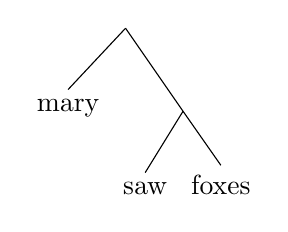
\begin{tikzpicture}
        \Tree [ mary [ saw foxes ] ]
      \end{tikzpicture}
    \end{center}
    And the denotation is:
    $$\exists p.\forall x.p(x)\supset(\mathbf{fox}(x)\land\mathbf{past}(\mathbf{see}(\text{mary},x)))$$
  }
  \only<2>{%
    \textit{``John loves \underline{everyone}.''}
    \\[0.125\baselineskip]
    Given that the parse tree is:
    \\[1\baselineskip]
    \begin{center}
      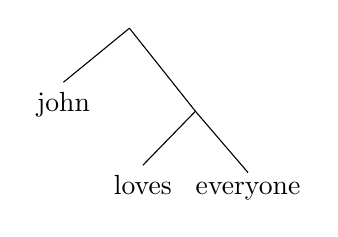
\begin{tikzpicture}
        \Tree [ john [ loves everyone ] ]
      \end{tikzpicture}
    \end{center}
    And the denotation is:
    $$\forall x.\mathbf{person}(x)\supset\mathbf{love}(\text{john},x)$$
  }
  \note{%
    It seems that the meaning of ``everyone'' is taking scope over the
    surrounding expressions.
  }
  \vfill
\end{frame}

\begin{frame}
  \frametitle{Scope Ambiguity}
  \textit{``\underline{A professor} talked to \underline{every student}.''}
  \\[0.125\baselineskip]
  Given that the parse tree is:
  \\[1\baselineskip]
  \begin{center}
    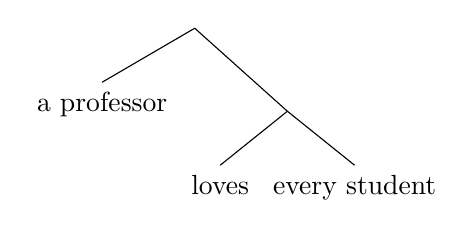
\begin{tikzpicture}
      \Tree [ {a professor} [ loves {every student} ] ]
    \end{tikzpicture}
  \end{center}
  And the denotation is:
  \begin{center}
    $\exists x.\mathbf{professor}(x)\land(\forall
    y.\mathbf{student}(y)\supset\mathbf{talk}(x,y))$
    \\
    $\forall y.\mathbf{student}(y)\supset(\exists
    x.\mathbf{professor}(x)\land\mathbf{talk}(x,y))$
  \end{center}
  \vfill
\end{frame}

\begin{frame}
  \frametitle{Scope Islands}
  \textit{``Mary \underline{said} \underline{everyone} left.''}
  \\[0.125\baselineskip]
  Given that the parse tree is:
  \\[1\baselineskip]
  \begin{center}
    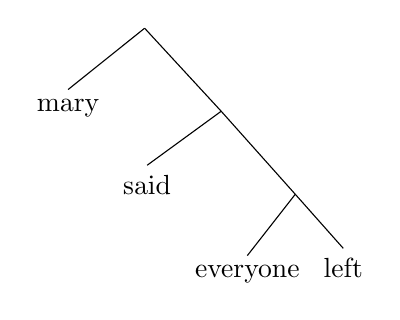
\begin{tikzpicture}
      \Tree [ mary [ said [ everyone left ] ] ]
    \end{tikzpicture}
  \end{center}
  \begin{minipage}{0.5\linewidth}
    And the denotation is:
    $$\mathbf{said}(\text{mary},\forall x.\mathbf{left}(x))$$
  \end{minipage}%
  \begin{minipage}{0.5\linewidth}
    And definitely isn't:
    $$\forall x.\mathbf{said}(\text{mary},\mathbf{left}(x))$$
  \end{minipage}
  \vfill
\end{frame}

\begin{frame}
  \frametitle{What could we do \textit{right now}?}
  \vfill
  \begin{itemize}
  \item
    Use higher order functions, but:
    \begin{itemize}
    \item[--] many different types
      \begin{itemize}
      \item
        $\S\impl(\NP\impr\S)$,
        $((\NP\impr\S)\impl\NP)\impr(\NP\impr\S)$,
        \ldots
      \end{itemize}
    \end{itemize}
  \item
    Use a continuation monad, but:
    \begin{itemize}
    \item[--] only \textit{one} interpretation, so no scope ambiguity
    \item[--] can only take scope at the top-level
    \item[--] can not be delimited
    \end{itemize}
    \note{%
      We do not want our semantic calculus to be ambiguous, so any
      ambiguity must arise from structural properties.
    }
  \item
    Use delimited continuations, but:
    \begin{itemize}
    \item[--] again, only \textit{one} interpretation
    \item[--] is not a monad, but an indexed monad, which has
      \textit{three arguments}, so should be reflected in the
      syntactic calculus
    \end{itemize}
  \end{itemize}
  \vfill
\end{frame}

\begin{frame}
  \frametitle{Quantifier Raising and NL\textsubscript{IBC}}
  \centering
  \vfill
  \only<1>{%
    \(\!
    \begin{aligned}
      \text{Structure}&^+\;&Γ&\coloneqq\ldots\vsep\I\vsep\B\vsep\C
    \end{aligned}
    \)
    \\[1\baselineskip]
    \begin{pfbox}
      \AXC{$\struct{A}\prod\I\fCenter Δ$} \RightLabel{L\I}
      \UIC{$\struct{A}\fCenter Δ$}
    \end{pfbox}
    \begin{pfbox}
      \AXC{$Γ\fCenter\struct{B}$} \RightLabel{R\I}
      \UIC{$Γ\prod\I\fCenter\struct{B}$}
    \end{pfbox}
    \\[1\baselineskip]
    \begin{pfbox}
      \AXC{$Γ_1\prod(Γ_2\prod Γ_3)\fCenter Δ$}
      \doubleLine\RightLabel{\B}
      \UIC{$Γ_2\prod((\B\prod Γ_1)\prod Γ_3)\fCenter Δ$}
    \end{pfbox}
    \begin{pfbox}
      \AXC{$(Γ_1\prod Γ_2)\prod Γ_3\fCenter Δ$}
      \doubleLine\RightLabel{\C}
      \UIC{$Γ_1\prod((\C\prod Γ_2)\prod Γ_3)\fCenter Δ$}
    \end{pfbox}
  }
  \only<2>{%
    \begin{pfbox}[0.7]
      \AXC{}\RightLabel{Ax}\UIC{$\struct{\S}\fCenter\struct{{\color{red}\S}}$}
      \AXC{$
        \struct{\NP}\prod
        \struct{(\NP\impr\S)\impl\NP}\prod
        \struct{{\color{red}\NP}}
        \fCenter
        \struct{{\color{red}\S}}$}
      \RightLabel{Res$\prod\impr$}
      \UIC{$
        \struct{(\NP\impr\S)\impl\NP}\prod
        \struct{{\color{red}\NP}}
        \fCenter
        \struct{\NP}\impr\struct{{\color{red}\S}}$}
      \RightLabel{Res$\prod\impr$}
      \UIC{$
        \struct{{\color{red}\NP}}
        \fCenter
        \struct{(\NP\impr\S)\impl\NP}\impr
        \struct{\NP}\impr
        \struct{{\color{red}\S}}$}
      \RightLabel{R\I}
      \UIC{$
        \struct{{\color{red}\NP}}\prod\I
        \fCenter
        \struct{(\NP\impr\S)\impl\NP}\impr
        \struct{\NP}\impr
        \struct{{\color{red}\S}}$}
      \RightLabel{Res$\impr\prod$}
      \UIC{$
        \struct{(\NP\impr\S)\impl\NP}\prod(\struct{{\color{red}\NP}}\prod\I)
        \fCenter
        \struct{\NP}\impr
        \struct{{\color{red}\S}}$}
      \RightLabel{\B}
      \UIC{$
        \struct{{\color{red}\NP}}\prod
        ((\B\prod\struct{(\NP\impr\S)\impl\NP})\prod\I)
        \fCenter
        \struct{\NP}\impr
        \struct{{\color{red}\S}}$}
      \RightLabel{Res$\prod\impr$}
      \UIC{$
        \struct{\NP}\prod
        (\struct{{\color{red}\NP}}\prod
        ((\B\prod\struct{(\NP\impr\S)\impl\NP})\prod\I))
        \fCenter
        \struct{{\color{red}\S}}$}
      \RightLabel{\B}
      \UIC{$
        \struct{{\color{red}\NP}}\prod
        ((\B\prod\struct{\NP})\prod
        ((\B\prod\struct{(\NP\impr\S)\impl\NP})\prod\I))
        \fCenter
        \struct{{\color{red}\S}}$}
      \RightLabel{Res$\prod\impr$}
      \UIC{$
        ((\B\prod\struct{\NP})\prod
        ((\B\prod\struct{(\NP\impr\S)\impl\NP})\prod\I))
        \fCenter
        \struct{{\color{red}\NP}}\impr
        \struct{{\color{red}\S}}$}
      \RightLabel{R$\impr$}
      \UIC{$
        ((\B\prod\struct{\NP})\prod
        ((\B\prod\struct{(\NP\impr\S)\impl\NP})\prod\I))
        \fCenter
        \struct{{\color{red}\NP\impr\S}}$}
      \RightLabel{L$\impl$}
      \BIC{$
        \struct{{\color{red}\S\impl(\NP\impr\S)}}
        \fCenter
        \struct{\S}\impl
        ((\B\prod\struct{\NP})\prod
        ((\B\prod\struct{(\NP\impr\S)\impl\NP})\prod\I))$}
      \RightLabel{Res$\impl\prod$}
      \UIC{$
        \struct{{\color{red}\S\impl(\NP\impr\S)}}\prod
        ((\B\prod\struct{\NP})\prod
        ((\B\prod\struct{(\NP\impr\S)\impl\NP})\prod\I))
        \fCenter
        \struct{\S}$}
      \RightLabel{$\B'$}
      \UIC{$
        \struct{\NP}\prod
        (\struct{{\color{red}\S\impl(\NP\impr\S)}}\prod
        ((\B\prod\struct{(\NP\impr\S)\impl\NP})\prod\I))
        \fCenter
        \struct{\S}$}
      \RightLabel{Res$\prod\impr$}
      \UIC{$
        \struct{{\color{red}\S\impl(\NP\impr\S)}}\prod
        ((\B\prod\struct{(\NP\impr\S)\impl\NP})\prod\I)
        \fCenter
        \struct{\NP}\impr
        \struct{\S}$}
      \RightLabel{$\B'$}
      \UIC{$
        \struct{(\NP\impr\S)\impl\NP}\prod
        (\struct{{\color{red}\S\impl(\NP\impr\S)}}\prod\I)
        \fCenter
        \struct{\NP}\impr
        \struct{\S}$}
      \RightLabel{Res$\impr\prod$}
      \UIC{$
        \struct{{\color{red}\S\impl(\NP\impr\S)}}\prod\I
        \fCenter
        \struct{(\NP\impr\S)\impl\NP}\impr
        \struct{\NP}\impr
        \struct{\S}$}
      \RightLabel{L\I}
      \UIC{$
        \struct{{\color{red}\S\impl(\NP\impr\S)}}
        \fCenter
        \struct{(\NP\impr\S)\impl\NP}\impr
        \struct{\NP}\impr
        \struct{\S}$}
      \RightLabel{Res$\prod\impr$}
      \UIC{$
        \struct{(\NP\impr\S)\impl\NP}\prod
        \struct{{\color{red}\S\impl(\NP\impr\S)}}
        \fCenter
        \struct{\NP}\impr
        \struct{\S}$}
      \RightLabel{Res$\prod\impr$}
      \UIC{$
        \struct{\NP}\prod
        \struct{(\NP\impr\S)\impl\NP}\prod
        \struct{{\color{red}\S\impl(\NP\impr\S)}}
        \fCenter
        \struct{\S}$}
    \end{pfbox}
  }
  \only<3>{%
    \begin{pfbox}[0.7]
      \AXC{}\RightLabel{Ax}\UIC{$\struct{\S}\fCenter\struct{{\color{red}\S}}$}
      \AXC{$
        \struct{\NP}\prod
        \struct{(\NP\impr\S)\impl\NP}\prod
        \struct{{\color{red}\NP}}
        \fCenter
        \struct{{\color{red}\S}}$}
      \noLine\UIC{\vphantom{$($}$\vdots$\vphantom{$)$}}
      \noLine\UIC{$
        \struct{{\color{red}\NP}}\prod
        ((\B\prod\struct{\NP})\prod
        ((\B\prod\struct{(\NP\impr\S)\impl\NP})\prod\I))
        \fCenter
        \struct{{\color{red}\S}}$}
      \RightLabel{R$\impr$}
      \UIC{$
        ((\B\prod\struct{\NP})\prod
        ((\B\prod\struct{(\NP\impr\S)\impl\NP})\prod\I))
        \fCenter
        \struct{{\color{red}\NP\impr\S}}$}
      \RightLabel{L$\impl$}
      \BIC{$
        \struct{{\color{red}\S\impl(\NP\impr\S)}}\prod
        ((\B\prod\struct{\NP})\prod
        ((\B\prod\struct{(\NP\impr\S)\impl\NP})\prod\I))
        \fCenter
        \struct{\S}$}
      \noLine\UIC{\vphantom{$($}$\vdots$\vphantom{$)$}}
      \noLine\UIC{$
        \struct{\NP}\prod
        \struct{(\NP\impr\S)\impl\NP}\prod
        \struct{{\color{red}\S\impl(\NP\impr\S)}}
        \fCenter
        \struct{\S}$}
    \end{pfbox}
  }
  \only<4>{%
    \begin{pfbox}[0.7]
      \noLine\AXC{\vphantom{$($}$\vdots$\vphantom{$)$}}
      \noLine\UIC{$
        \struct{{\color{green}\S\impl(\NP\impr\S)}}\prod
        (\B\prod\struct{{\color{red}\S\impl(\NP\impr\S)}}\prod
        (\C\prod(\B\prod\B)\prod\I)\prod
        (\B\prod\struct{(\NP\impr\S)\impl\NP})\prod\I
        \fCenter\struct{\S}$}
      \noLine\UIC{\vphantom{$($}$\vdots$\vphantom{$)$}}
      \noLine\UIC{$
        \struct{{\color{red}\S\impl(\NP\impr\S)}}\prod
        (\B\prod\struct{{\color{green}\S\impl(\NP\impr\S)}})\prod
        (\B\prod\struct{(\NP\impr\S)\impl\NP})\prod\I
        \fCenter\struct{\S}$}
      \noLine\UIC{\vphantom{$($}$\vdots$\vphantom{$)$}}
      \noLine\UIC{$
        \struct{{\color{green}\S\impl(\NP\impr\S)}}\prod
        \struct{(\NP\impr\S)\impl\NP}\prod
        \struct{{\color{red}\S\impl(\NP\impr\S)}}
        \fCenter\struct{\S}$}
    \end{pfbox}
  }
  \only<5>{%
    \(\!
    \begin{aligned}
      \text{Structure}&^+\;&Γ &\coloneqq \ldots\vsep Γ_1\hprod Γ_2\vsep\I\vsep\B\vsep\C\\
      \text{Structure}&^-\;&Δ &\coloneqq \ldots\vsepΔ\himplΓ\vsepΓ\himprΔ
    \end{aligned}
    \)
    \\[1\baselineskip]
    (copy of rules for $\{\impr,\prod,\impl\}$ for $\{\himpr,\hprod,\himpl\}$)
    \\[1\baselineskip]
    \begin{pfbox}
      \AXC{$\struct{A}\hprod\I\fCenter Δ$}
      \RightLabel{L\I}
      \UIC{$\struct{A}\fCenter Δ$}
    \end{pfbox}
    \begin{pfbox}
      \AXC{$Γ\fCenter\struct{B}$}
      \RightLabel{R\I}
      \UIC{$Γ\hprod\I\fCenter\struct{B}$}
    \end{pfbox}
    \\[1\baselineskip]
    \begin{pfbox}
      \AXC{$Γ_1\prod(Γ_2\hprod Γ_3)\fCenter Δ$}
      \doubleLine\RightLabel{\B}
      \UIC{$Γ_2\hprod((\B\prod Γ_1)\prod Γ_3)\fCenter Δ$}
    \end{pfbox}
    \begin{pfbox}
      \AXC{$(Γ_1\hprod Γ_2)\prod Γ_3\fCenter Δ$}
      \doubleLine\RightLabel{\C}
      \UIC{$Γ_1\hprod((\C\prod Γ_2)\prod Γ_3)\fCenter Δ$}
    \end{pfbox}
  }
  \only<6>{%
    \begin{pfbox}[0.7]
      \noLine\AXC{\vphantom{$($}$\vdots$\vphantom{$)$}}
      \noLine\UIC{$
        \struct{{\color{red}(\NP\impr\S)\impl\NP}}\hprod
        (\B\prod\struct{\NP})\prod
        ((\C\prod\I)\prod\struct{\NP})$}
      \noLine\UIC{\vphantom{$($}$\vdots$\vphantom{$)$}}
      \noLine\UIC{$
        \struct{\NP}\prod
        \struct{{\color{red}(\NP\impr\S)\impl\NP}}\prod
        \struct{\NP}
        \fCenter\struct{\S}$}
    \end{pfbox}
    \begin{pfbox}[0.7]
      \noLine\AXC{\vphantom{$($}$\vdots$\vphantom{$)$}}
      \noLine\UIC{$
        ((\struct{\NP}{\;\color{red}\hprod\;\I}){\;\color{red}\hprod\;\I})\prod
        \struct{\NP\impr\S}\prod
        \fCenter\struct{\S}$}
      \noLine\UIC{\vphantom{$($}$\vdots$\vphantom{$)$}}
      \noLine\UIC{$
        (\struct{\NP}{\;\color{red}\hprod\;\I})\prod
        \struct{\NP\impr\S}\prod
        \fCenter\struct{\S}$}
      \noLine\UIC{\vphantom{$($}$\vdots$\vphantom{$)$}}
      \noLine\UIC{$
        \struct{\NP}\prod
        \struct{\NP\impr\S}\prod
        \fCenter\struct{\S}$}
    \end{pfbox}
  }
  \only<7>{%
    \(\!
    \begin{aligned}
      \text{Type}     &  \;&A,B&\coloneqq \ldots\vsep\qr[A]\\
      \text{Structure}&^+\;&Γ  &\coloneqq \ldots\vsep Γ_1\hprod Γ_2\vsep\I\vsep\B\vsep\C\\
      \text{Structure}&^-\;&Δ   &\coloneqq \ldots\vsepΔ\himplΓ\vsepΓ\himprΔ
    \end{aligned}
    \)
    \\[1\baselineskip]
    (copy of rules for $\{\impr,\prod,\impl\}$ for $\{\himpr,\hprod,\himpl\}$)
    \\[1\baselineskip]
    \begin{pfbox}
      \AXC{$\struct{A}\hprod\I\fCenter Δ$}
      \RightLabel{L\I}
      \UIC{$\struct{\qr[A]}\fCenter Δ$}
    \end{pfbox}
    \begin{pfbox}
      \AXC{$Γ\fCenter\struct{B}$}
      \RightLabel{R\I}
      \UIC{$Γ\hprod\I\fCenter\struct{\qr[B]}$}
    \end{pfbox}
    \begin{pfbox}
      \AXC{$Γ\fCenter Δ$}
      \RightLabel{$\I^-$}
      \UIC{$Γ\hprod\I\fCenter Δ$}
    \end{pfbox}
    \\[1\baselineskip]
    \begin{pfbox}
      \AXC{$Γ_1\prod(Γ_2\hprod Γ_3)\fCenter Δ$}
      \doubleLine\RightLabel{\B}
      \UIC{$Γ_2\hprod((\B\prod Γ_1)\prod Γ_3)\fCenter Δ$}
    \end{pfbox}
    \begin{pfbox}
      \AXC{$(Γ_1\hprod Γ_2)\prod Γ_3\fCenter Δ$}
      \doubleLine\RightLabel{\C}
      \UIC{$Γ_1\hprod((\C\prod Γ_2)\prod Γ_3)\fCenter Δ$}
    \end{pfbox}
  }
  \only<8>{%
    \begin{pfbox}[0.7]
      \AXC{}\RightLabel{Ax}\UIC{$\struct{\S}\fCenter\struct{{\color{red}\S}}$}
      \AXC{$
        \struct{\NP}\prod
        \struct{(\NP\impr\S)\impl\NP}\prod
        \struct{{\color{red}\NP}}
        \fCenter
        \struct{{\color{red}\S}}$}
      \noLine\UIC{\vphantom{$($}$\vdots$\vphantom{$)$}}
      \noLine\UIC{$
        \struct{{\color{red}\NP}}\hprod
        ((\B\prod\struct{\NP})\prod
        ((\B\prod\struct{(\NP\impr\S)\impl\NP})\prod\I))
        \fCenter
        \struct{{\color{red}\S}}$}
      \RightLabel{R$\impr$}
      \UIC{$
        ((\B\prod\struct{\NP})\prod
        ((\B\prod\struct{(\NP\impr\S)\impl\NP})\prod\I))
        \fCenter
        \struct{{\color{red}\NP\himpr\S}}$}
      \RightLabel{L$\impl$}
      \BIC{$
        \struct{{\color{red}\S\himpl(\NP\himpr\S)}}\hprod
        ((\B\prod\struct{\NP})\prod
        ((\B\prod\struct{(\NP\himpr\S)\himpl\NP})\prod\I))
        \fCenter
        \struct{\S}$}
      \noLine\UIC{\vphantom{$($}$\vdots$\vphantom{$)$}}
      \noLine\UIC{$
        \struct{\NP}\prod
        \struct{(\NP\impr\S)\impl\NP}\prod
        \struct{{\color{red}\qr[\S\himpl(\NP\himpr\S)]}}
        \fCenter
        \struct{\S}$}
    \end{pfbox}
  }
  \vfill
\end{frame}



\begin{frame}
  \frametitle{Quantifier Raising and Scope Islands}
  \only<1>{%
    \vfill
    \begin{center}
      \(\!
      \begin{aligned}
        \text{Type}     &  \;&A,B&\coloneqq \ldots\vsep\di A\vsep\sq A\\
        \text{Structure}&^+\;&Γ  &\coloneqq \ldots\vsep\langle Γ\rangle\\
        \text{Structure}&^-\;&Δ &\coloneqq \ldots\vsep[Δ]
      \end{aligned}
      \)
      \\[1\baselineskip]
      \begin{pfbox}
        \AXC{$\langle\struct{A}\rangle\fCenter Δ$} \RightLabel{L$\di$}
        \UIC{$\struct{\di A}\fCenter Δ$}
      \end{pfbox}
      \begin{pfbox}
        \AXC{$Γ\fCenter\struct{B}$} \RightLabel{R$\di$}
        \UIC{$\langle Γ\rangle\fCenter\struct{\di B}$}
      \end{pfbox}
      \\[1\baselineskip]
      \begin{pfbox}
        \AXC{$\struct{A}\fCenter Δ$} \RightLabel{L$\di$}
        \UIC{$\struct{\sq A}\fCenter[Δ]$}
      \end{pfbox}
      \begin{pfbox}
        \AXC{$Γ\fCenter[\struct{B}]$} \RightLabel{R$\sq$}
        \UIC{$Γ\fCenter\struct{\sq B}$}
      \end{pfbox}
      \\[1\baselineskip]
      \begin{pfbox}
        \AXC{$Γ\fCenter[Δ]$} \doubleLine\RightLabel{Res$\sq\di$}
        \UIC{$\langle Γ\rangle\fCenter Δ$}
      \end{pfbox}
    \end{center}
    \vfill
  }
  \only<2>{%
    \textit{``Mary \underline{said} \underline{everyone} left.''}
    \vfill
    \begin{center}
      \begin{pfbox}
        \noLine\AXC{\vphantom{$($}$\vdots$\vphantom{$)$}}
        \noLine\UIC{$ \struct{\NP}\prod
          \struct{(\NP\impr\S)\impl\di\S}\prod
          \langle
          \struct{\qr[\S\himpl(\NP\himpr\S)]}\prod
          \struct{\NP\impr\S}
          \rangle
          \fCenter\struct{\S}$}
      \end{pfbox}
    \end{center}
    \vfill
  }
\end{frame}

\begin{frame}
  \frametitle{Future Work}
  \vfill
  \only<1>{%
    \centering
    {
      \color{gray}
      {Mary:NP see:TV.PAST fox:NP.PL}\\
      $\downarrow$\\
      \fbox{Syntactic}\\
      $\downarrow$\\
    }
    {Mary:NP [see:TV.PAST fox:NP.PL]}\\
    $\downarrow$\\
    \fbox{Semantic}\\
    $\downarrow$\\
    $\exists p.\forall x.p(x)\supset(\mathbf{fox}(x)\land
    \mathbf{past}(\mathbf{see}(\text{mary},x)))$
  }
  \only<2->{%
    \onslide<2->{%
      Forward-Chaining Proof Search:
      \begin{itemize}
      \item[--] generate all possible sentences;
      \item[--] filter on the sentences with the right word order.
      \end{itemize}
    }
    \onslide<3->{%
      Weak vs. Strong quantifiers:
      \begin{itemize}
      \item[--] different quantifiers show different behaviour
        w.r.t. scope islands.
      \end{itemize}
    }
  }
  \vfill
\end{frame}

\begin{frame}
  \centering
  \vfill
  \LARGE
  Bonus Slides
  \vfill
\end{frame}

\begin{frame}
  \frametitle{L$\!{\himpl}{\downarrow}$ and R${\himpr}{\uparrow}$ as
    derivable rules}
  \centering
  \vfill
  \only<1-2>{%
    \begin{pfbox}[0.9]
      \AXC{}\RightLabel{Ax}\UIC{$\struct{\S}\fCenter\struct{{\color{red}\S}}$}
      \AXC{$
        \struct{\NP}\prod
        \struct{(\NP\impr\S)\impl\NP}\prod
        \struct{{\color{red}\NP}}
        \fCenter
        \struct{{\color{red}\S}}$}
      \only<1>{\noLine\UIC{\vphantom{$($}$\vdots$\vphantom{$)$}}\noLine}%
      \only<2>{\RightLabel{${\uparrow}$}}%
      \UIC{$
        \struct{{\color{red}\NP}}\hprod
        ((\B\prod\struct{\NP})\prod
        ((\B\prod\struct{(\NP\impr\S)\impl\NP})\prod\I))
        \fCenter
        \struct{{\color{red}\S}}$}
      \RightLabel{R$\himpr$}
      \UIC{$
        ((\B\prod\struct{\NP})\prod
        ((\B\prod\struct{(\NP\impr\S)\impl\NP})\prod\I))
        \fCenter
        \struct{{\color{red}\NP\himpr\S}}$}
      \RightLabel{L$\himpl$}
      \BIC{$
        \struct{{\color{red}\S\himpl(\NP\himpr\S)}}\hprod
        ((\B\prod\struct{\NP})\prod
        ((\B\prod\struct{(\NP\impr\S)\impl\NP})\prod\I))
        \fCenter
        \struct{\S}$}
      \only<1>{\noLine\UIC{\vphantom{$($}$\vdots$\vphantom{$)$}}\noLine}%
      \only<2>{\RightLabel{${\downarrow}$}}%
      \UIC{$
        \struct{\NP}\prod
        \struct{(\NP\impr\S)\impl\NP}\prod
        \struct{{\color{red}\qr[\S\himpl(\NP\himpr\S)]}}
        \fCenter
        \struct{\S}$}
    \end{pfbox}
  }
  \only<3>{%
    \begin{pfbox}[0.9]
      \AXC{}\RightLabel{Ax}\UIC{$\struct{\S}\fCenter\struct{{\color{red}\S}}$}
      \AXC{$
        \struct{\NP}\prod
        \struct{(\NP\impr\S)\impl\NP}\prod
        \struct{{\color{red}\NP}}
        \fCenter
        \struct{{\color{red}\S}}$}
      \RightLabel{R${\himpr}{\uparrow}$}
      \UIC{$
        ((\B\prod\struct{\NP})\prod
        ((\B\prod\struct{(\NP\impr\S)\impl\NP})\prod\I))
        \fCenter
        \struct{{\color{red}\NP\himpr\S}}$}
      \RightLabel{L${\himpl}{\downarrow}$}
      \BIC{$
        \struct{\NP}\prod
        \struct{(\NP\impr\S)\impl\NP}\prod
        \struct{{\color{red}\qr[\S\himpl(\NP\himpr\S)]}}
        \fCenter
        \struct{\S}$}
    \end{pfbox}
  }
  \only<4>{%
  \(\!
    \begin{aligned}
      \text{Context}\;Σ\coloneqq\Box\vsepΣ\prodlΔ\vsepΓ\prodrΣ
    \end{aligned}
  \)
  \\[2\baselineskip]
  \(\!
    \begin{aligned}
      \Box      [Γ]&\mapsto Γ\\
      (Σ\prodlΔ)[Γ]&\mapsto (Σ[Γ]\prod Δ)\\
      (Δ\prodrΣ)[Γ]&\mapsto (Δ\prod Σ[Γ])
    \end{aligned}
    \quad
    \begin{aligned}
      &\text{Trace}(\Box)    &&\mapsto \I\\
      &\text{Trace}(Σ\prodlΔ)&&\mapsto ((\C\prod Σ[Γ])\prod Δ)\\
      &\text{Trace}(Δ\prodrΣ)&&\mapsto ((\B\prod Δ)\prod Σ[Γ])
    \end{aligned}
  \)
  \\[2\baselineskip]
  \begin{pfbox}[0.9]
    \AXC{$\struct{C}\fCenterΔ$}
    \AXC{$\text{Trace}(Σ)\fCenter\struct{B}$}
    \RightLabel{L$\!{\himpl}{\downarrow}$}
    \BIC{$Σ[\struct{\qr[C\himpl B]}]\fCenter Δ$}
  \end{pfbox}
  \begin{pfbox}[0.9]
    \AXC{$Σ[\struct{A}]\fCenter\struct{B}$}
    \RightLabel{R${\himpr}{\uparrow}$}
    \UIC{$\text{Trace}(Σ)\fCenter\struct{A\impr B}$}
  \end{pfbox}
  }
  \vfill
\end{frame}

\end{document}

%%% Local Variables:
%%% mode: latex
%%% TeX-master: t
%%% End:
